\documentclass[a4paper,10pt]{jsarticle}

% 数式
\usepackage{amsmath,amsfonts}
\usepackage{bm}
% 画像
\usepackage[dvipdfmx]{graphicx}
\usepackage{here}

\usepackage{listingsutf8,jlisting} %日本語のコメントアウトをする場合jlistingが必要
%ここからソースコードの表示に関する設定
\lstset{
  basicstyle={\ttfamily},
  identifierstyle={\small},
  commentstyle={\smallitshape},
  keywordstyle={\small\bfseries},
  ndkeywordstyle={\small},
  stringstyle={\small\ttfamily},
  frame={tb},
  breaklines=true,
  columns=[l]{fullflexible},
  numbers=left,
  xrightmargin=0zw,
  xleftmargin=3zw,
  numberstyle={\scriptsize},
  stepnumber=1,
  numbersep=1zw,
  lineskip=-0.5ex
}

\begin{document}

\title{オペレーティングシステム演習問題1}
\author{坪井正太郎(101830245)}
\date{\today}
\maketitle
\section{問題1}
\subsection{server.cと,client.cの実行}
以下のように実行されて,正しく動作している。
\begin{lstlisting}[caption={server実行結果},label={server1}]
  $ ./server
  Ready.
  Waiting for a connection...
  Connection established.
  Sending the message...
  Waiting for a connection...
\end{lstlisting}

\begin{lstlisting}[caption={client実行結果},label={client1}]
  $ ./client
  Connecting to the server...
  Connected.
  Message from the server:

  Hello!
  Good-by!!
\end{lstlisting}


\subsection{両プログラム実行時のフローチャート}
図\ref{フローチャート}に示した。


\section{問題2}
変更はソースコード\ref{server2.c}に示す。
「//変更部!!!」で囲った部分を変更した。
入力先の領域をchar*256分確保して,fscanfで入力を読んだ。

以下のコマンドを実行し,結果を得た。
2回目の実行も正しく動作している。
\begin{lstlisting}[caption={server2},label={server2}]
  $ ./server
  Ready.
  Waiting for a connection...
  Connection established.
  Enter your message
  hello^D
  Waiting for a connection...
  Connection established.
  Enter your message
  goodbye^D
  Waiting for a connection...  
\end{lstlisting}

\begin{lstlisting}[caption={client},label={client2}]
  $ ./client
  Connecting to the server...
  Connected.
  Message from the server:

  hello

  Finished receiving.

  $ ./client
  Connecting to the server...
  Connected.
  Message from the server:

  goodbye

  Finished receiving.
\end{lstlisting}


\section{問題3}
変更は,ソースコード\ref{server3.c} に示す。
親プロセスからforkして並列にループ内を実行した。

以下のような実行結果になった。
4つのクライアントから,並列にアクセスしたところ,サーバ側で4つ同時に接続が確立されていることがわかる。

\begin{lstlisting}[caption={server3},label={server3}]
  ./server
  Ready.
  Waiting for a connection...
  Connection established.
  Waiting for a connection...
  Enter your message
  Connection established.
  Waiting for a connection...
  Enter your message
  Connection established.
  Waiting for a connection...
  Enter your message
  Connection established.
  Waiting for a connection...
  Enter your message
  hello1
  hello2
  hello3
  hello4  
\end{lstlisting}

\begin{lstlisting}[caption={client3},label={client3-1}]
  ./client & ./client & ./client & ./client
  Connecting to the server...
  Connected.
  Message from the server:
  
  Connecting to the server...
  Connected.
  Message from the server:
  
  Connecting to the server...
  Connected.
  Message from the server:
  
  Connecting to the server...
  Connected.
  Message from the server:
  hello1
  
  Finished receiving.
  hello2
  
  Finished receiving.
  hello3
  
  Finished receiving.
  hello4
  
  Finished receiving.  
\end{lstlisting}

\begin{figure}[H]
  \centering
  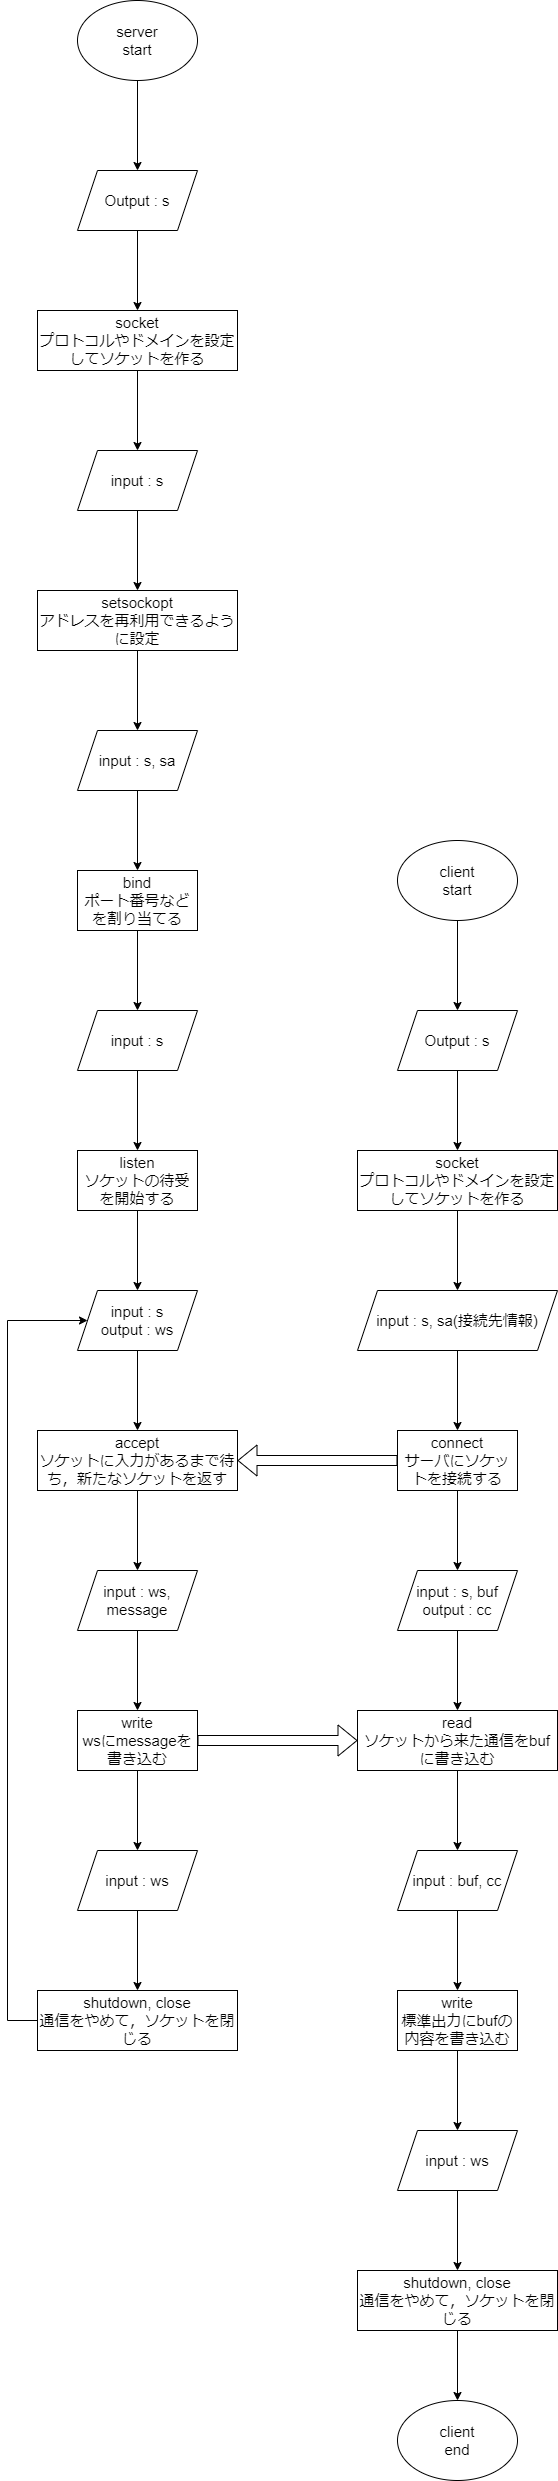
\includegraphics[width=5cm]{./01.png}
  \caption{フローチャート}
  \label{フローチャート}
\end{figure}

\lstinputlisting[caption=server2.c,label=server2.c]{./server2.c}
\lstinputlisting[caption=server3.c,label=server3.c]{./server3.c}


\end{document}
